\addcontentsline{toc}{chapter}{Haggai}
% Safely inserts your illustration full-bleed on its own page.
% This completely bypasses the page builder, headers, and geometry bugs!
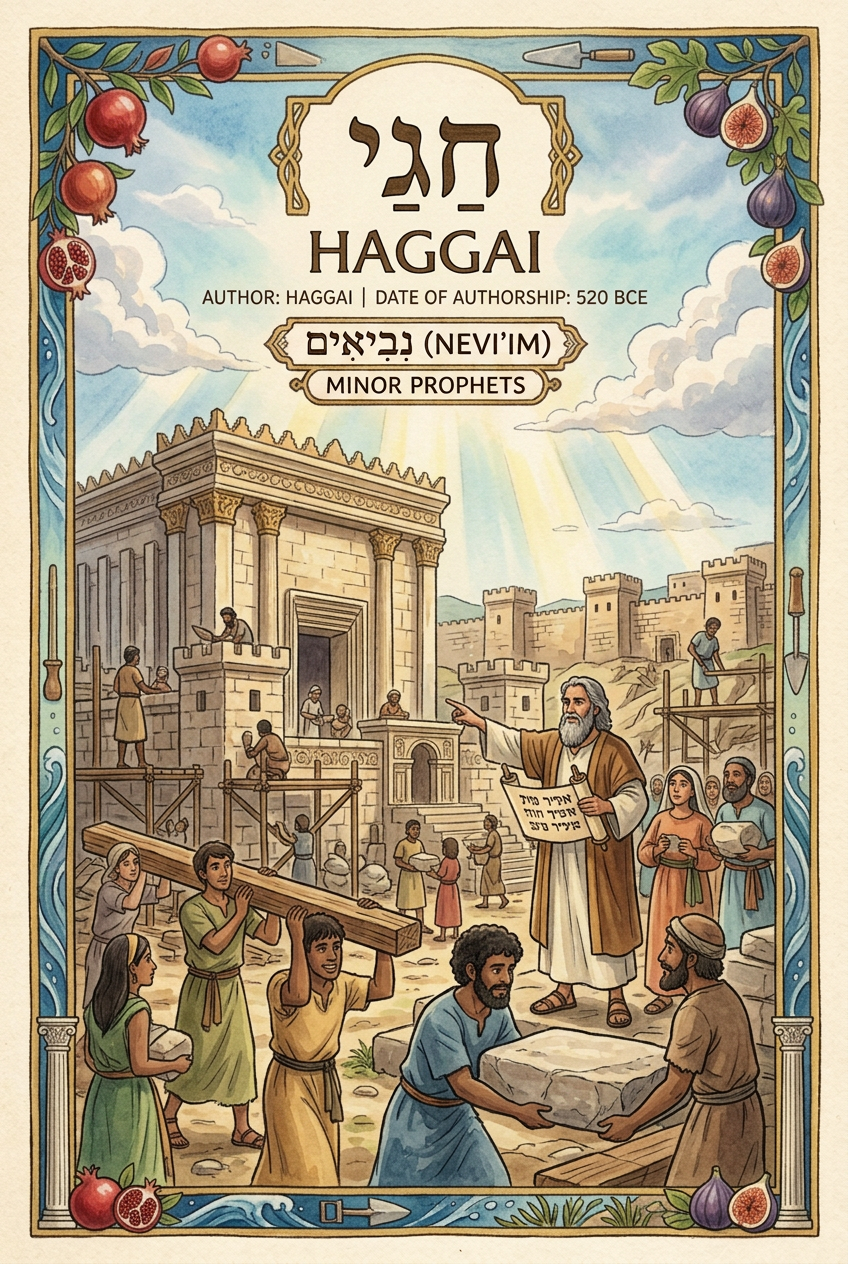
\includepdf[pages=1, fitpaper=false, width=\paperwidth, height=\paperheight, , keepaspectratio=false]{images/divider2/haggai_2.png}
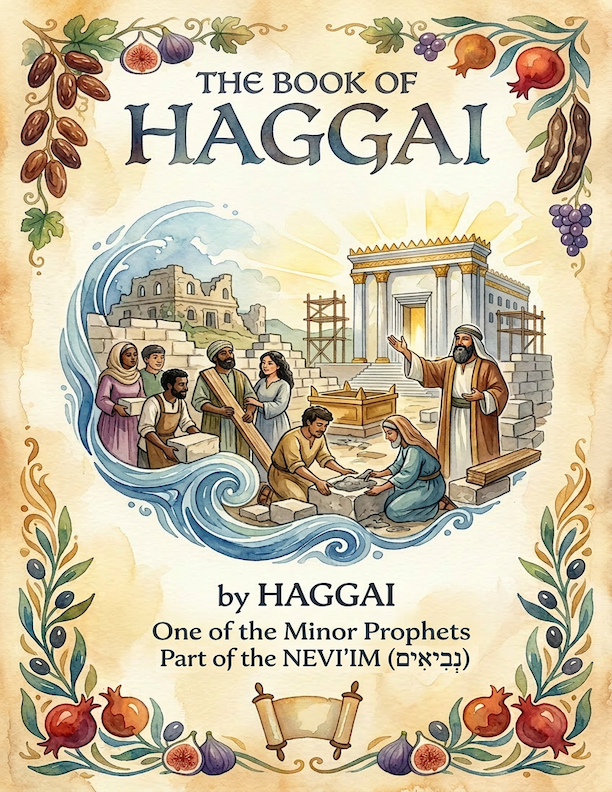
\includepdf[pages=1, fitpaper=false, width=\paperwidth, height=\paperheight, , keepaspectratio=false]{images/divider1/haggai.png}

\includepdf[pages=1, fitpaper=false, width=\paperwidth, height=\paperheight, , keepaspectratio=false]{images/8.5x11-Dot-Grid.png}

\includepdf[pages=1, fitpaper=false, width=\paperwidth, height=\paperheight, , keepaspectratio=false]{images/8.5x11-Dot-Grid.png}
\mybook{Haggai}
\vspace{-1.36in}


\mychapter{} \myverse*{}In the second year of Darius the king, in the sixth month, in the first day of the month, the LORD’s\footnote{1:1 When rendered in ALL CAPITAL LETTERS, “LORD” or “GOD” is the translation of God’s Proper Name.} word came by Haggai the prophet, to Zerubbabel the son of Shealtiel, governor of Judah, and to Joshua the son of Jehozadak, the high priest, saying, \myverse{}“This is what the LORD of Hosts says: These people say, ‘The time hasn’t yet come, the time for the LORD’s house to be built.’ ”


\myverse{}Then the LORD’s word came by Haggai the prophet, saying, \myverse{}“Is it a time for you yourselves to dwell in your paneled houses, while this
house lies waste? \myverse{}Now therefore this is what the LORD of Hosts says: ‘Consider your ways. \myverse{}You have sown much, and bring in little. You eat, but you don’t have enough. You drink, but you aren’t filled with drink. You clothe yourselves, but no one is warm; and he who earns wages earns wages to put them into a bag with holes in it.’


\myverse{}“This is what the LORD of Hosts says: ‘Consider your ways. \myverse{}Go up to the mountain, bring wood, and build the house. I will take pleasure in it, and I will be glorified,” says the LORD. \myverse{}“You looked for much, and, behold,\footnote{1:9 “Behold”, from “הִנֵּה”, means look at, take notice, observe, see, or gaze at. It is often used as an interjection.} it came to little; and when you brought it home, I blew it away. Why?” says the LORD of Hosts, “Because of my house that lies waste, while each of you is busy with his own house. \myverse{}Therefore for your sake the heavens withhold the dew, and the earth withholds its fruit. \myverse{}I called for a drought on the land, on the mountains, on the grain, on the new wine, on the oil, on that which the ground produces, on men, on livestock, and on all the labor of the hands.”


\myverse{}Then Zerubbabel the son of Shealtiel and Joshua the son of Jehozadak,
the high priest, with all the remnant of the people, obeyed the LORD their God’s\footnote{1:12 The Hebrew word rendered “God” is “אֱלֹהִ֑ים” (Elohim).} voice, and the words of Haggai the prophet, as the LORD their God had sent him; and the people feared the LORD.

\myverse{}Then Haggai, the LORD’s messenger, spoke the LORD’s message to
the people, saying, “I am with you,” says the LORD.


\myverse{}The LORD stirred up the spirit of Zerubbabel the son of Shealtiel, governor of Judah, and the spirit of Joshua the son of Jehozadak, the high priest, and the spirit of all the remnant of the people; and they came and worked on the house of the LORD of Hosts, their God, \myverse{}in the twenty-fourth day of the month, in the sixth month, in the second year of Darius the king.


% HAGGAI 2
\mychapter{} \myverse*{}In the seventh month, in the twenty-first day of the month, the LORD’s word came by Haggai the prophet, saying, \myverse{}“Speak now to Zerubbabel the son of Shealtiel, governor of Judah, and to Joshua the son of Jehozadak, the high priest, and to the remnant of the people, saying, \myverse{}‘Who is left among you who saw this house in its former glory? How do you see it now? Isn’t it in your eyes as nothing? \myverse{}Yet now be strong, Zerubbabel,’ says the LORD. ‘Be strong, Joshua son of Jehozadak, the high priest. Be strong, all you people of the land,’ says the LORD, ‘and work, for I am with you,’ says the LORD of Hosts. \myverse{}This is the word that I covenanted with you when you came out of Egypt, and my Spirit lived among you. ‘Don’t be afraid.’ \myverse{}For this is what the LORD of Hosts says: ‘Yet once more, it is a little while, and I will shake the heavens, the earth, the sea, and the dry land; \myverse{}and I will shake all nations. The treasure of all nations will come, and I will fill this house with glory, says the LORD of Hosts. \myverse{}The silver is mine, and the gold is mine,’ says the LORD of Hosts. \myverse{}‘The latter glory of this house will be greater than the former,’ says the LORD of Hosts; ‘and in this place I will give peace,’ says the LORD of Hosts.”

 \myverse{}In the twenty-fourth day of the ninth month, in the second year of Darius, the LORD’s word came by Haggai the prophet, saying, \myverse{}“The LORD of Hosts says: Ask now the priests concerning the law, saying, \myverse{}‘If someone carries holy meat in the fold of his garment, and with his fold
touches bread, stew, wine, oil, or any food, will it become holy?’ ”

The priests answered, “No.”


\myverse{}Then Haggai said, “If one who is unclean by reason of a dead
body touches any of these, will it be unclean?”

The priests answered, “It will be unclean.”


\myverse{}Then Haggai answered, “ ‘So is this people, and so is this nation
before me,’ says the LORD; ‘and so is every work of their hands. That which they offer there is unclean. \myverse{}Now, please consider from this day and backward, before a stone was laid on a stone in the LORD’s temple. \myverse{}Through all that time, when one came to a heap of twenty measures, there were only ten. When one came to the wine vat to draw out fifty, there were only twenty. \myverse{}I struck you with blight, mildew, and hail in all the work of your hands; yet you didn’t turn to me,’ says the LORD. \myverse{}‘Consider, please, from this day and backward, from the twenty-fourth day of the ninth month, since the day that the foundation of the LORD’s temple was laid, consider it. \myverse{}Is the seed yet in the barn? Yes, the vine, the fig tree, the pomegranate, and the olive tree haven’t produced. From today I will bless you.’ ”

 \myverse{}The LORD’s word came the second time to Haggai in the twenty-fourth day of the month, saying, \myverse{}“Speak to Zerubbabel, governor of Judah, saying, ‘I will shake the heaven and the earth. \myverse{}I will overthrow the throne of kingdoms. I will destroy the strength of the kingdoms of the nations. I will overthrow the chariots and those who ride in them. The horses and their riders will come down, everyone by the sword of his brother. \myverse{}In that day, says the LORD of Hosts, I will take you, Zerubbabel my servant, the son of Shealtiel,’ says the LORD, ‘and will make you like a signet ring, for I have chosen you,’ says the LORD of Hosts.”


